\documentclass[11pt, titlepage]{article}
\usepackage{amsmath,amsthm,amssymb}
\usepackage{hyperref, pgf, tikz}
\usepackage{fancyhdr}
\usetikzlibrary{arrows}
\usepackage[margin=1.25in]{geometry}
\usepackage{graphicx}                     
\pagestyle{fancy}
\usepackage{array}
\usepackage{indentfirst}
%\usepackage{wrapfig}

\lhead{Lab \#1}
\rhead{\thepage}
\cfoot{}

\title{The Measurement of Resistance: Ammeter-Voltmeter Methods and Wheatstone Bridge Method \\ \ \\ \large Lab \#1}
\author{Name: Avery Karlin \\ Partner: Ethan Chang}
\date{}
\begin{document}

\maketitle

\begin{center}
\LARGE The Measurement of Resistance: Ammeter-Voltmeter Methods and Wheatstone Bridge Method
\end{center}

\section*{Objective}
The objective of the lab is to measure the resistance of unknown resistors by means of both the Wheatstone bridge of balancing the resistance of both sides of the bridge, and by a combined ammeter and voltmeter.

\section*{Introduction}
The measuring of resistance can be done by several methods, the first of which depends on Ohm's Law, stating $R = \frac{V}{I}$. On the other hand, since the voltmeter, placed in parallel such that the voltage is equal, takes away a portion of the current, or because the ammeter, placed in series such that the current is equal, takes away a portion of the voltage, the measurement is not exact. If the resistance of the voltmeter greatly exceeds that of the resistor, it will not interfere, while if the resistance of the ammeter is vastly less, it will not interfere. Otherwise, for the voltmeter impacting the current, $R = \frac{V}{I_R} = \frac{V}{I - I_v} = \frac{V}{I - \frac{V}{R_V}}$, where $I_R$ is the voltage through the resistor, $I_v$ is the current through the voltmeter, and $R_V$ is the resistance of the voltmeter. For the ammeter impacting the voltage, $R = \frac{V_R}{I} = \frac{V - V_A}{I} = \frac{V - R_AI}{I} = \frac{V}{I} - R_A$.

As a result, it can be seen that as the voltmeter resistance approaches infinity, the resistance approaches $\frac{V}{I}$ for the former case, such that it plays no effect, and likewise, as the ammeter resistance approaches zero, the resistance approaches the same, such that there is no effect. This is due to the fact that as voltmeter resistance is infinite, the resistance through the other path is so far below, that all the current moves through there, while the current through the voltmeter is negligable. As the ammeter resistance approaches 0, no voltage is lost passing through it as a result, since it acts like a normal wire, thus having no effect.

\begin{figure}[h]
\centering
\hspace*{0cm}
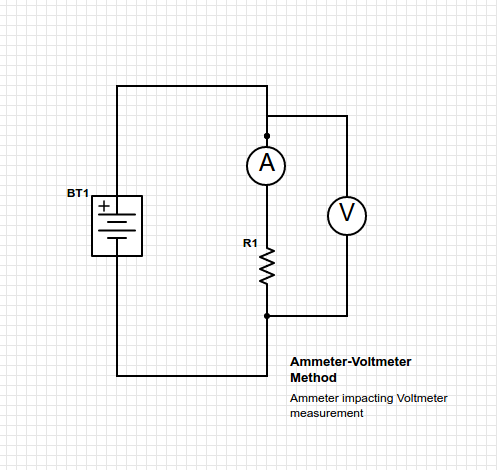
\includegraphics[scale=1, angle=0]{circuit1.jpg}
\vspace*{0cm}
\end{figure}

\begin{figure}[h]
\centering
\hspace*{0cm}
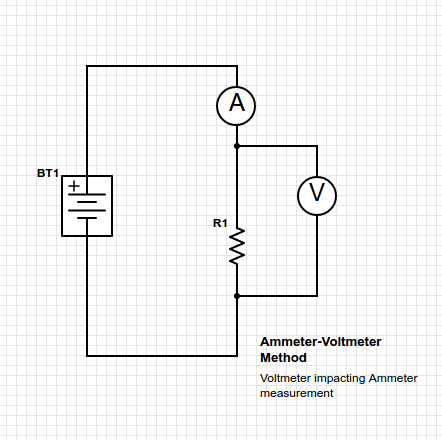
\includegraphics[scale=1, angle=0]{circuit2.jpg}
\vspace*{0cm}
\end{figure}

The other method of calculating resistance is the Wheatstone Bridge method, which can be done either by the slide-wire method or the four-resistor method. The four resistor method places two known resistors in series on one side of the bridge, and a variable resistor and the unknown on the other side, with a galvanometer/ammeter connected from the center of both sides. The variable resistor can then be modified such that the first resistor on each side has an equal voltage to the other ($I_1R_1 = I_2R_V$) and the second on each has an equal voltage ($I_2R_1 = I_2R_X$), where $R_V$ is the variable resistance and $R_X$ is the unknown resistor. Thus, at that point $R_X = \frac{R_2R_V}{R_1}$.

\begin{figure}[h]
\centering
\hspace*{0cm}
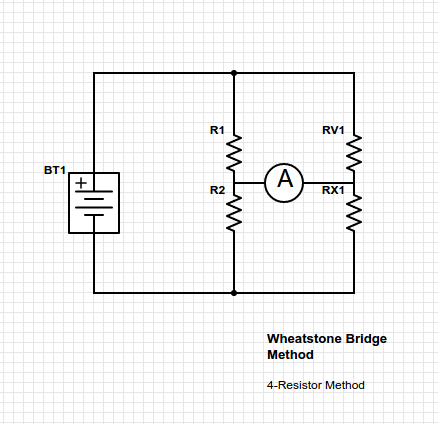
\includegraphics[scale=1, angle=0]{circuit3.jpg}
\vspace*{0cm}
\end{figure}

The slide-wire method uses a slide wire resistor instead of the two known resistors and a known resistor instead of the variable one. As a result, since the resistance of each part of the slide wire resistor is proportional to the length, it can similarly be found that $R_X = \frac{L_2R_K}{L_1}$, where $R_K$ is the known resistor, $L_1$ is the length of the wire parallel to the known resistor, and $L_2$ is the length parallel to the unknown resistor.

\section*{Procedures and Results}

First, the Ammeter-Voltmeter methods are used with a small resistor, first creating a circuit such that the ammeter reading is slightly higher than actual, second so that the voltmeter reading is slightly higher than actual, with an additional variable resistor, a rheostat in this case using only one of the resistors, separate from the resistor being measured, in series. The resistance of the ammeter and the voltmeter can be separately measured by an ohmmeter, so that they can be taken into account. The voltage and current across the resistor can thus be found as well. It is then taken for three different rheostat resistances, such that the voltage and current through the unknown resistor varies. It is then redone by the same means for a large resistor.

\begin{figure}[h]
\centering
\hspace*{0cm}
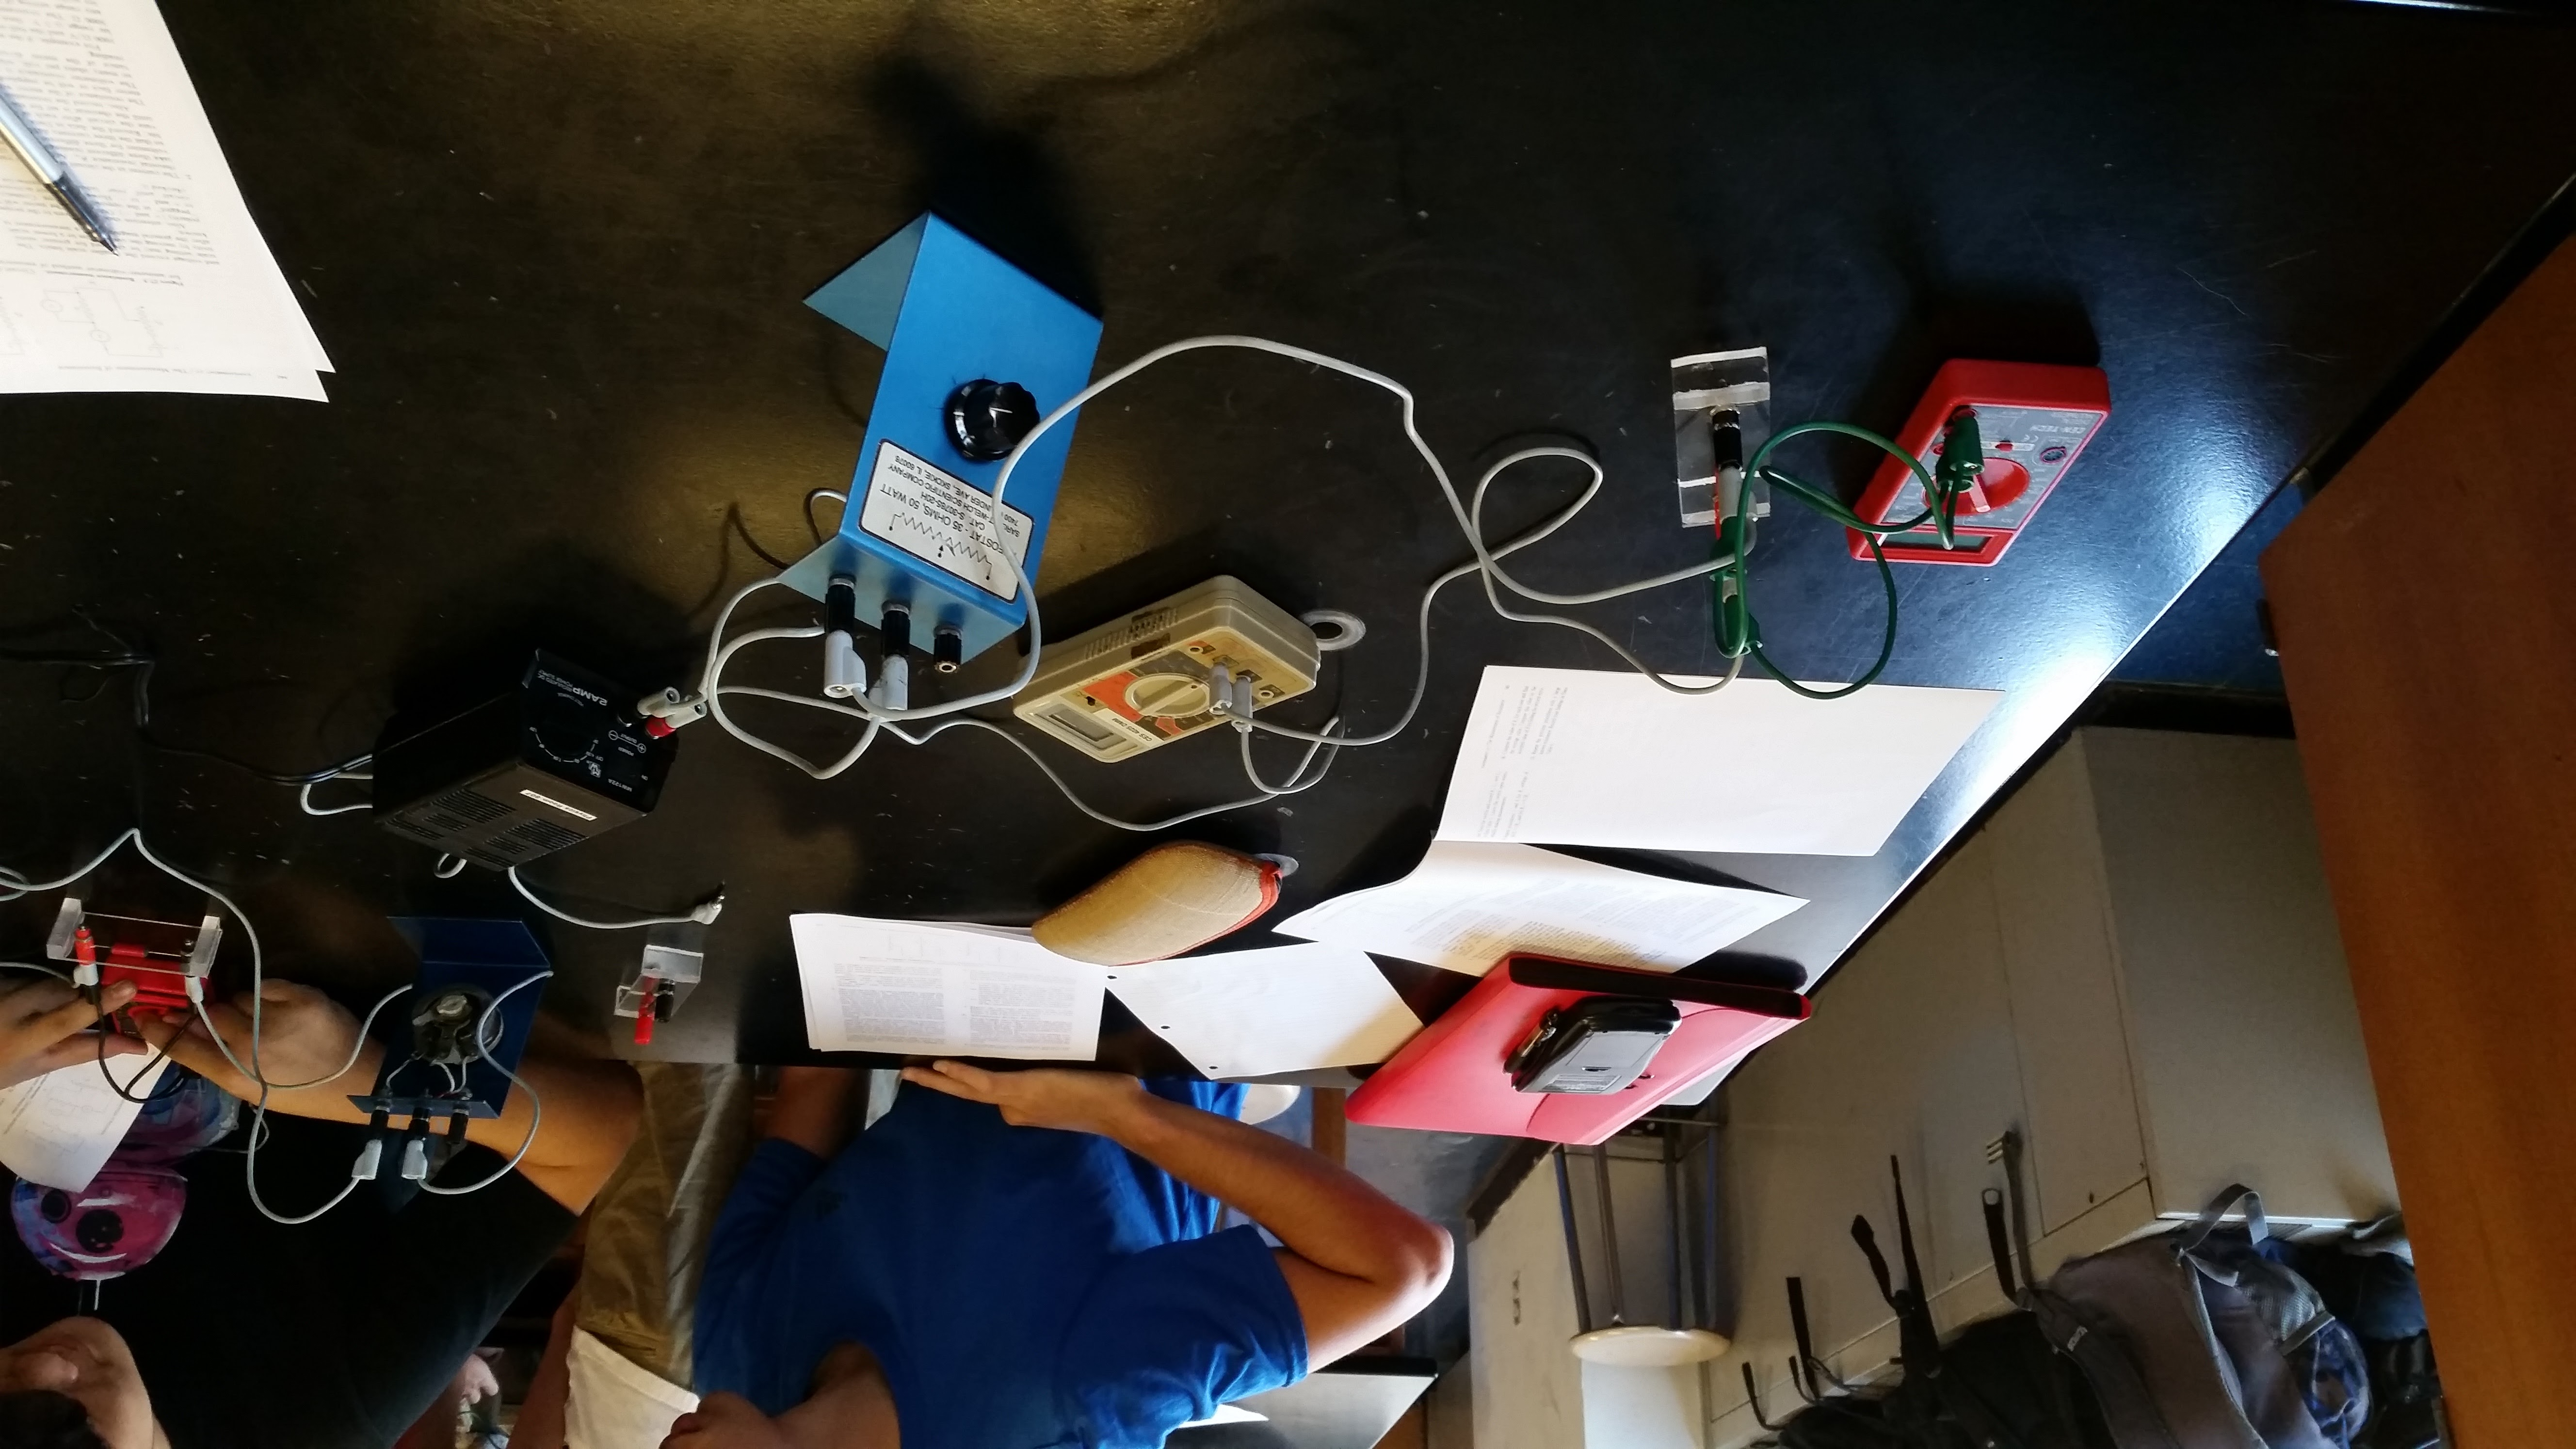
\includegraphics[scale=0.12, angle=90]{lab11.jpg}
\vspace*{0cm}
\end{figure}

\begin{figure}[h]
\centering
\hspace*{0cm}
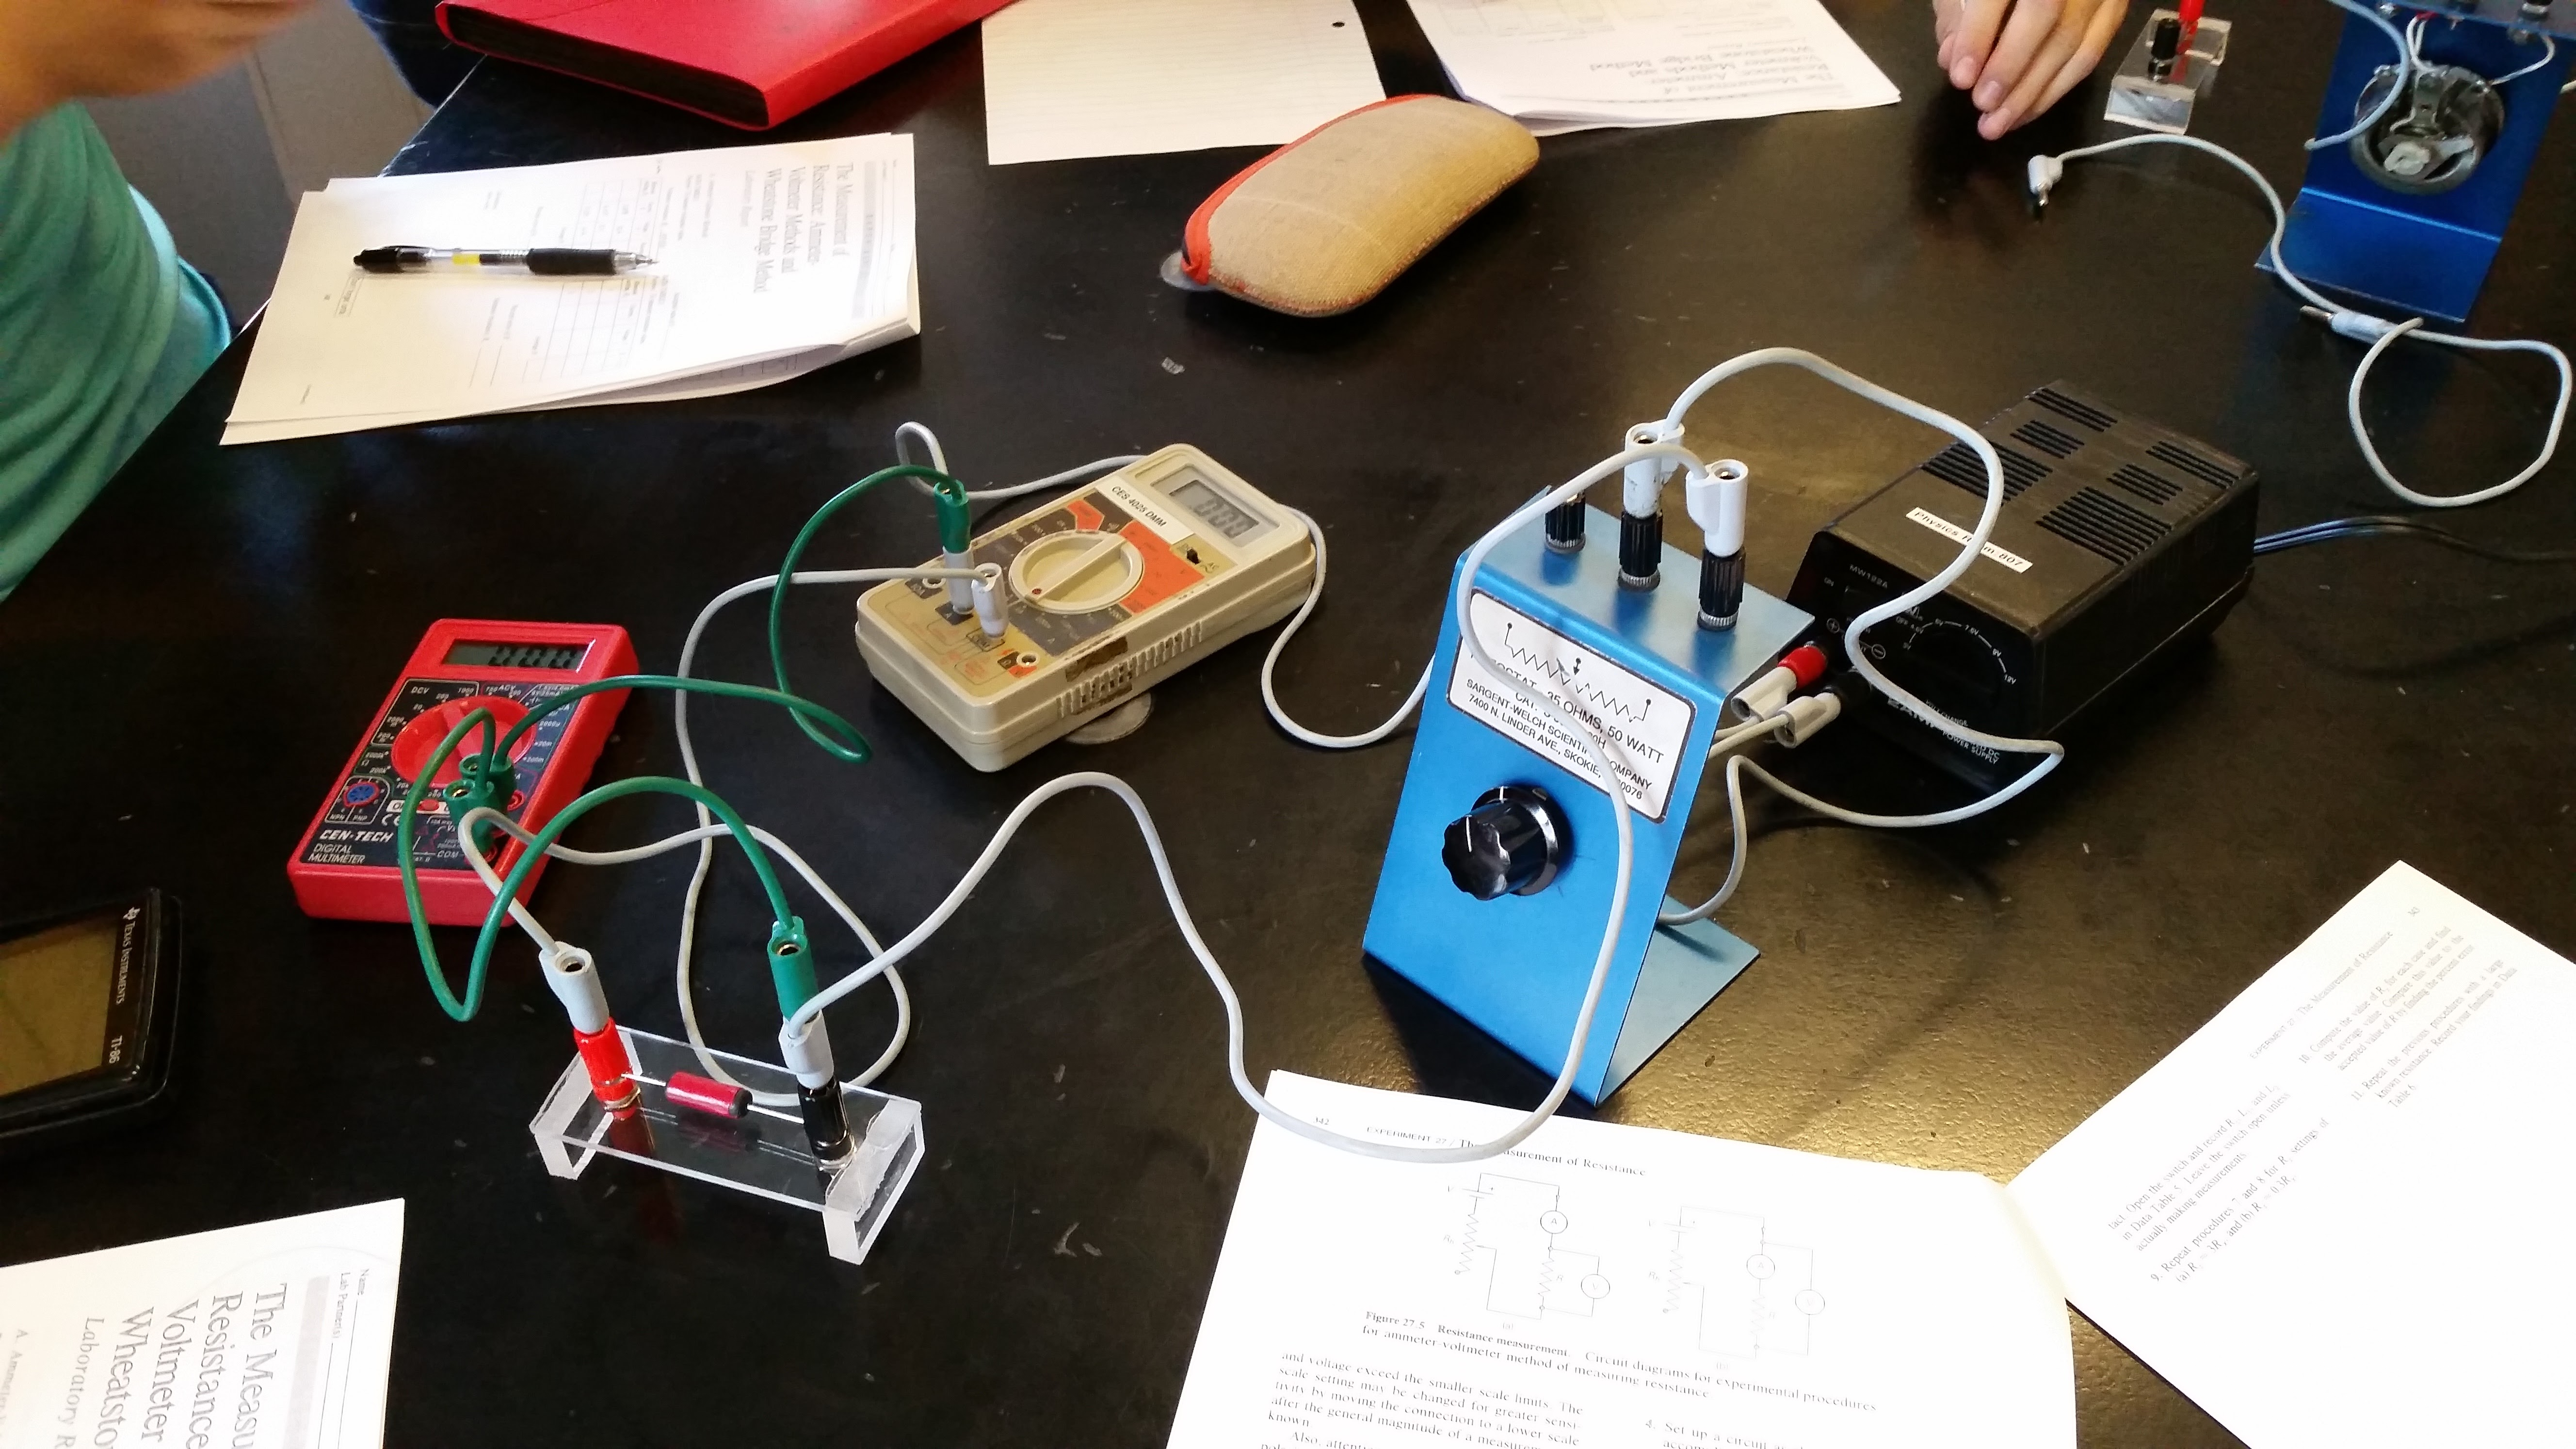
\includegraphics[scale=0.12, angle=270]{lab12.jpg}
\vspace*{0cm}
\end{figure}

The slide-wire form of the Wheatstone Bridge is then made in a variation, with a rheostat used as the two unknown resistors, due to acting as two varying resistors in series, with a divider between, similar to a slide-wire. It is measured for some small and large unknown resistor, taken for three different known resistors with each part of the rheostat resistance measured by an ohmmeter when there is no current passing through the bridge, measured by an ammeter.

\begin{figure}[h]
\centering
\hspace*{0cm}
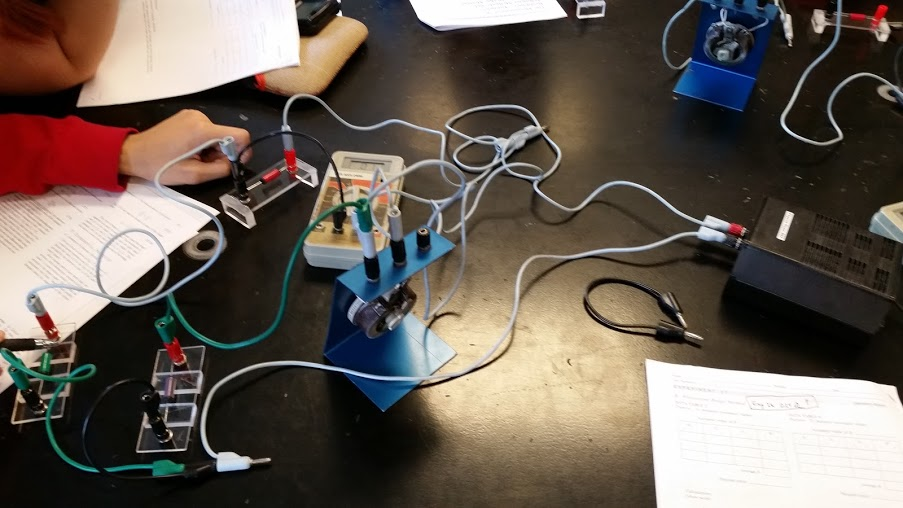
\includegraphics[scale=0.7, angle=270]{lab13.jpg}
\vspace*{0cm}
\end{figure}

\underline{Small Resistor:}
\begin{center}
$$R_V \text{(Voltmeter Resistance)}= 1 \Omega$$
$$R_X \text{(Expected Resistance)}= 50.2 \Omega$$
\begin{tabular}
{|m{9em}|m{7em}|m{7em}|m{7em}|}
\hline
Rheostat Setting & 1 & 2 & 3 \\
\hline
Current, I (A) & 0.048 & 0.039 & 0.031 \\
\hline
Voltage, V (V) & 2.6 & 2.1 & 1.6 \\
\hline
\end{tabular}
\end{center}

\begin{center}
$$R_A \text{(Ammeter Resistance)}= 0.48 \Omega$$
$$R_X \text{(Expected Resistance)}= 50.2 \Omega$$
\begin{tabular}
{|m{9em}|m{7em}|m{7em}|m{7em}|}
\hline
Rheostat Setting & 1 & 2 & 3 \\
\hline
Current, I (A) & 0.048 & 0.039 & 0.032 \\
\hline
Voltage, V (V) & 2.6 & 2.1 & 1.6 \\
\hline
\end{tabular}
\end{center}

\underline{Large Resistor:}
\begin{center}
$$R_V \text{(Voltmeter Resistance)}= 1 \Omega$$
$$R_X \text{(Expected Resistance)}= 74.7 \Omega$$
\begin{tabular}
{|m{9em}|m{7em}|m{7em}|m{7em}|}
\hline
Rheostat Setting & 1 & 2 & 3 \\
\hline
Current, I (A) & 0.033 & 0.029 & 0.024 \\
\hline
Voltage, V (V) & 2.6 & 2.3 & 1.9 \\
\hline
\end{tabular}
\end{center}

\begin{center}
$$R_A \text{(Ammeter Resistance)}= 0.48 \Omega$$
$$R_X \text{(Expected Resistance)}= 74.7 \Omega$$
\begin{tabular}
{|m{9em}|m{7em}|m{7em}|m{7em}|}
\hline
Rheostat Setting & 1 & 2 & 3 \\
\hline
Current, I (A) & 0.032 & 0.029 & 0.021 \\
\hline
Voltage, V (V) & 2.6 & 2.3 & 1.7 \\
\hline
\end{tabular}
\end{center}

\underline{Wheatstone Bridge:}
\begin{center}
$$R_X \text{(Expected Resistance)}= 25.6 \Omega$$
\begin{tabular}
{|m{9em}|m{7em}|m{7em}|m{7em}|}
\hline
Known Resistor, $R_K (\Omega)$ & 50.2 & 74.6 & 25.6 \\
\hline
Varying Resistor 1, $R_1 (\Omega)$ & 24.2 & 26.1 & 17.5 \\
\hline
Varying Resistor 2, $R_2 (\Omega)$ & 12.8 & 9.4 & 17.5 \\
\hline
\end{tabular}
\end{center}

\begin{center}
$$R_X \text{(Expected Resistance)}= 74.7 \Omega$$
\begin{tabular}
{|m{9em}|m{7em}|m{7em}|m{7em}|}
\hline
Known Resistor, $R_K (\Omega)$ & 25.6 & 50.2 & 74.6 \\
\hline
Varying Resistor 1, $R_1 (\Omega)$ & 8.7 & 13.9 & 17 \\
\hline
Varying Resistor 2, $R_2 (\Omega)$ & 26.1 & 21.2 & 17.9 \\
\hline
\end{tabular}
\end{center}

\section*{Discussion}
Sample calculations for the non-measured data are as shown using the formulas found above:

\underline{Small Resistor:}
\begin{center}
\begin{tabular}
{|m{9em}|m{7em}|m{7em}|m{7em}|}
\hline
Rheostat Setting & 1 & 2 & 3 \\
\hline
Resistance, R $(\Omega)$ & & & \\
\hline
\end{tabular}
\\Average Resistance ($\Omega$) =
\\Percent Error = 
\end{center}

\begin{center}
\begin{tabular}
{|m{9em}|m{7em}|m{7em}|m{7em}|}
\hline
Rheostat Setting & 1 & 2 & 3 \\
\hline
Resistance, R $(\Omega)$ & & & \\
\hline
\end{tabular}
\\Average Resistance ($\Omega$) = 
\\Percent Error = 
\end{center}

\underline{Large Resistor:}
\begin{center}
\begin{tabular}
{|m{9em}|m{7em}|m{7em}|m{7em}|}
\hline
Rheostat Setting & 1 & 2 & 3 \\
\hline
Resistance, R $(\Omega)$ & & & \\
\hline
\end{tabular}
\\Average Resistance ($\Omega$) = 
\\Percent Error = 
\end{center}

\begin{center}
\begin{tabular}
{|m{9em}|m{7em}|m{7em}|m{7em}|}
\hline
Rheostat Setting & 1 & 2 & 3 \\
\hline
Resistance, R $(\Omega)$ & & & \\
\hline
\end{tabular}
\\Average Resistance ($\Omega$) =
\\Percent Error = 
\end{center}

\underline{Wheatstone Bridge:}
\begin{center}
\begin{tabular}
{|m{9em}|m{7em}|m{7em}|m{7em}|}
\hline
Rheostat Setting & 1 & 2 & 3 \\
\hline
Resistance, R $(\Omega)$ & & & \\
\hline
\end{tabular}
\\Average Resistance = 
\\Percent Error = 
\end{center}

\begin{center}
\begin{tabular}
{|m{9em}|m{7em}|m{7em}|m{7em}|}
\hline
Rheostat Setting & 1 & 2 & 3 \\
\hline
Resistance, R $(\Omega)$ & & & \\
\hline
\end{tabular}
\\Average Resistance = 
\\Percent Error = 
\end{center}


Our percent error was fairly high for the first set of data, especially as the mass was lower, most likely indicating an issue with the time measurement, as it was faster at the start, at which points the percent of error was far higher. 

Other sources of error that could have occured was within the pulley mechanism itself, estimating the frictional mass manually, which created room for error, and it assumes that the pulley itself worked as intended, although there was the chance of it slipping or catching at any point. In addition, there is the possibility of drag force slowing the measured acceleratin, which is consistent with the data, except in the 1st and 5th trial.

Finally, the equations themselves assumed a point mass, while in actuality, as the masses got higher, they became less and less point-like in shape, interfering in the data.

\section*{Conclusion}

The acceleration as the mass on each side before frictional mass was added increased from 0.05 to 0.15 to 0.25 to 0.35, went from 1.015 $m/s^2$ with 58.59\% error, to 0.359 $m/s^2$ with 23.62 \% error, to 0.196 $m/s^2$ with 27.4 \% error, to 0.105 $m/s^2$ with 19.7\% error.

The acceleration as the mass difference increased from 2 g to 6 g to 10 g to 20 g, went from 0.0196 $m/s^2$ with 12 \% error, to 0.0715 $m/s^2$ with 18.5 \% error, to 0.137 $m/s^2$ with 13.3 \% error, to 0.283 $m/s^2$ with 15.01 \% error. 

\end{document}
